\documentclass[letterpaper]{article} % DO NOT CHANGE THIS
\usepackage[submission]{aaai25}  % DO NOT CHANGE THIS
\usepackage{times}  % DO NOT CHANGE THIS
\usepackage{helvet}  % DO NOT CHANGE THIS
\usepackage{courier}  % DO NOT CHANGE THIS
\usepackage[hyphens]{url}  % DO NOT CHANGE THIS
\usepackage{graphicx} % DO NOT CHANGE THIS
\urlstyle{rm} % DO NOT CHANGE THIS
\def\UrlFont{\rm}  % DO NOT CHANGE THIS
\usepackage{natbib}  % DO NOT CHANGE THIS AND DO NOT ADD ANY OPTIONS TO IT
\usepackage{caption} % DO NOT CHANGE THIS AND DO NOT ADD ANY OPTIONS TO IT
\frenchspacing  % DO NOT CHANGE THIS
\setlength{\pdfpagewidth}{8.5in} % DO NOT CHANGE THIS
\setlength{\pdfpageheight}{11in} % DO NOT CHANGE THIS

\usepackage{amsmath}
\usepackage{algorithm}
\usepackage{algorithmic}
\usepackage{amsfonts} 
\usepackage{caption} %
\usepackage{subcaption}
\usepackage{amssymb}
\usepackage{fancybox}  
\usepackage[breakable]{tcolorbox}  
\usepackage{graphicx}
\usepackage{tcolorbox}  
\usepackage{mathptmx} 
\usepackage{amsmath}
\usepackage{xspace}
\usepackage{tabularx}
\usepackage{booktabs}
%
%               Personal Imports
%
\usepackage{multirow}
%
% Definitions.
% --------------------
\def\x{{\mathbf x}}
\def\L{{\cal L}}
\newcommand\mytop{\rule{0pt}{2ex}} % FOR FIRST DRAFT OF EXPERIMENTS TABLE CAN REMOVE IF WE REFORMAT
\newcommand\method{GETO-GNN\xspace}
\newcommand\graph{\mathcal{G}}
\newcommand\G{\mathcal{G}}
\newcommand\vertexSet{\mathcal{V}}
\newcommand\edgeSet{\mathcal{E}}
\newcommand\polylineSet{\mathcal{P}}
\newcommand\nodeSet{\mathcal{N}}
\newcommand\image{\mathbf{X}}
\newcommand\polyline{\mathbf{p}}
\newcommand{\matW}{\mathbf{W}}
\newcommand\msc{\mathbf{MSC}}
\newcommand\graphMSC{\mathcal{M}}
\newcommand\neighborPoly{\mathbf{q}}
\newcommand\Mspace{\mathbb{M}}
\newcommand\Rspace{\mathbb{R}}
\newcommand{\V}[1]{\mathbf{#1}}
\newcommand\MLP{\mathbf{MLP}}
\newcommand\PCA{\mathbf{PCA}}
\newcommand\concat{\mathbf{concat}}

\newcommand\subG{\mathcal{G}_{sb}}
\newcommand\supG{\mathcal{G}_{sp}}
\newcommand\subE{\mathbf{E}_{sb}}
\newcommand\supE{\mathbf{E}_{sp}}
\newcommand\subV{\mathbf{V}_{sb}}
\newcommand\supV{\mathbf{V}_{sp}}
\newcommand{\Nbr}[1]{\mathcal{N}(#1)}

\newcommand{\subNbr}[1]{\mathcal{N}_{sb}(#1)}
\newcommand{\supNbr}[1]{\mathcal{N}_{sp}(#1)}

\newcommand\iG{\mathbf{G}_{p_i}}
\newcommand\jG{\mathbf{G}_{p_j}}
\newcommand\iE{\mathbf{E}_{p_i}}
\newcommand\jE{\mathbf{E}_{p_j}}
\newcommand\iV{\mathbf{V}_{p_i}}
\newcommand\jV{\mathbf{V}_{p_j}}
\newcommand\iv{v_i}
\newcommand\jv{v_j}
\newcommand{\hk}[2]{h_{#1}^{#2}}
\newcommand{\iNbr}[1]{\mathcal{N}_{p_i}(#1)}
\newcommand{\jNbr}[1]{\mathcal{N}_{p_j}(#1)}

\newcommand\iW{\mathbf{W}_{i}}
\newcommand\jW{\mathbf{W}_{j}}
\newcommand*\imap{%
 \gamma_{p_i} }
 \newcommand*\jmap{%
 \gamma_{p_j} }

 \newcommand\Fo{$\text{F}_1$~}
 
\newcommand{\showcomment}{} % Comment this line to hide all comments in the document
\newcommand{\addcomment}[2]{\ifdefmacro{\showcomment}{{\textcolor{#1}{#2}}}{}}
\newcommand{\mh}[1]{\addcomment{red}{[Mark: #1]}}
%\newcommand{\addcomment}[2]{\ifdefmacro{\showcomment}{{\textcolor{#1}{#2}}}{}}

\definecolor{sc}{rgb}{0.6,0.30, 0.6}
\definecolor{seagreen}{rgb}{0.18, 0.55, 0.34}
%\newcommand{\scom}[1]{\addcomment{sc}{\red{\big[}{~ #1~}\red{\big]}}}
\newcommand{\samcom}[1]{\addcomment{blue}{[Sam: #1]}}

\definecolor{sn}{rgb}{0.3,0.60, 0.6}
\newcommand{\snote}[1]{\addcomment{seagreen}{{\red{\big[}~ #1~\red{\big]}}}} 


%%  To see bulleted section outlines
\newcommand\boxitem[1]{\begin{tcolorbox}[standard jigsaw,colframe=orange, opacityframe=0.5, opacityback=0.5, width=0.9\columnwidth, halign=flush left]{#1} \end{tcolorbox} }

%  To hide bulleted outlines
\newcommand{\hide}[1]{}
%\newcommand{\boxitem}[1]{\hide{#1}}


%colors
\newcommand{\blue}[1]{\addcomment{blue}{#1}}
\newcommand{\red}[1]{\addcomment{red}{#1}}
\newcommand{\yellow}[1]{\addcomment{yellow}{#1}}
\newcommand{\lightblue}[1]{\addcomment{cyan}{#1}}
\newcommand{\green}[1]{\addcomment{green}{#1}}
\newcommand{\purple}[1]{\addcomment{violet}{#1}}
\newcommand{\pink}[1]{\addcomment{magenta}{#1}}


\definecolor{orangebrown}{rgb}{0.5,0.35, 0.10}
\newcommand{\orangebrown}[1]{\addcomment{orangebrown}{#1}}
\definecolor{dorange}{rgb}{1.0,0.30, 0.0}
\newcommand{\dorange}[1]{\addcomment{dorange}{#1}}
\definecolor{redorange}{rgb}{0.9,0.50, 0.0}
\newcommand{\redorange}[1]{\addcomment{redorange}{#1}}
\definecolor{dyellow}{rgb}{0.75,0.7, 0.0}
\newcommand{\dyellow}[1]{\addcomment{dyellow}{#1}}
\definecolor{blonde}{rgb}{1.0, 0.60,0.0}
\newcommand{\blonde}[1]{\addcomment{blonde}{#1}}
\definecolor{Blue}{rgb}{0.0, 0.0, 1.0}
\newcommand{\Blue}[1]{\addcomment{Blue}{#1}}
\definecolor{lblue}{rgb}{0.25,0.35, 0.95}
\newcommand{\lblue}[1]{\addcomment{lblue}{#1}}
\definecolor{grey}{rgb}{0.3,0.33, 0.33}
\newcommand{\grey}[1]{\addcomment{grey}{#1}}
\definecolor{Green}{rgb}{0.0, 0.4, 0.0}
\newcommand{\Green}[1]{\addcomment{Green}{#1}}
\definecolor{lgreen}{rgb}{0.3, 0.9, 0.1}
\newcommand{\lgreen}[1]{\addcomment{lgreen}{#1}}
\definecolor{lorange}{rgb}{1.0,0.50, 0.0}
\newcommand{\lorange}[1]{\addcomment{lorange}{#1}}
\definecolor{springgreen}{rgb}{0.0, 0.9, 0.4}
\newcommand{\springgreen}[1]{\addcomment{springgreen}{#1}}


\title{Filtration Learning for Graph Neural Networks}

\author{Samuel Leventhal$^{\ddagger}$  \qquad Valerio Pascucci$^{\ddagger}$ \qquad
Mark Heimann$^{\dagger}$}

\affiliations{$^{\ddagger}$ University of Utah, Salt Lake City, UT, USA \\
$^{\dagger}$Lawrence Livermore National Laboratory, Livermore, CA, USA}

\begin{document}
\maketitle

 
\begin{abstract}
Graph neural networks (GNNs) are a powerful method of learning representations of graph-structured data. They excel at learning class-discriminative representations of nodes in homophilous graphs, where connecting nodes tend to belong to the same class. However, many graph neural networks struggle with heterophilous graphs whose nodes tend to connect to others of different classes since it has been shown that the heterophilous edges can muddy the message passing.  Inspired by this finding, we propose to design a topological filtration scheme for the graph based on the probability that a classifier predicts an edge is heterophilous. Using topological filtration based on predicted edge assignments, we can create an ordered sequence of subgraphs. As filtration helps track the evolution of graph connectivity and class connectivity over time, the resulting sequence of nested graphs captures the appearance and merging of connected components and cycles through heterophilous edges. We introduce two methodologies to exploit the sequence of graphs obtained through filtration to train a backbone GNN model. Both methodologies aim to reduce oversmoothing by enhancing the influence of early birth nodes in subgraphs with higher co-class connectivity. The first trains a GNN on each graph in the filtration sequence consecutively for a portion of the total training time, using embeddings from previous graphs to initialize node embeddings in subsequent graphs. The second approach uses a novel message passing scheme to pass messages jointly within each graph and between graph levels with common nodes. The second approach introduced further increases the impact of informative relationships while filtering out uninformative ones through a learnable attention scheme and node filter function for each graph level before multi-scale aggregation. Experiments show that our proposed method improves node classification accuracy on heterophilous and homophilous networks alike.

\iffalse
\mh{Too long and difficult to read for an abstract (this reads more like the introduction to a paper, although it should have paragraph breaks for that). Should be 1 short to medium length paragraph. Good abstract template you can use for an ML paper:
\\ Sentence 1: we're studying an important problem
\\ Sentence 2: powerful methods have been introduced to solve this problem (optional: they often work well because...)
\\ Sentence 3: alas, such methods suffer from a limitation
\\ Sentence 4: we have a great idea to fix this limitation
\\ Sentence 5: here is what our method does
\\ Sentence 6: experiments show that our method is good in this way(s) (be as specific as possible)
}
\fi

\end{abstract}

\section{Introduction}
Graphical representations offer an accessible and actionable means to express and expand our understanding of the world, from observed phenomena to abstract notions, by providing explanations or interpretations based on relationships and connections between elements, circumstances, and complex systems. Graph Neural Networks (GNNs) have emerged as a powerful tool for learning from graph structured data by generalizing the convolution operator to unstructured domains by leveraging message passing or neighborhood aggregation schemes to harness structural information. Recently, in graph machine learning, the classical task of node classification has demonstrated strong results when employing GNNs. 

Despite their potential, GNNs face several known challenges limiting their effectiveness and expressivity; of these obstacles, message passing networks schemes probably can not distinguish specific topologies, such as two triangles from a 6-cycle, and a leading known impediment to GNNs are graphs with high heterophily, namely, graphs whose edges predominantly adjoin nodes of disparate classes, which leads to oversmoothing~\cite{murphy2019relational,sato2021random,li2018deeper}. This paper introduces a graph learning methodology that addresses the limitations of conventional GNNs by offering a novel approach employing hierarchical GNNs-leveraging topological insights from persistent homology, namely persistence filtration, to reveal meaningful structure in graphs informed by class connectivity and allowing for a hierarchy of multilevel graph resolutions. 

The methodologies introduced here learn class relationships between nodes by first initializing edge embeddings from the combined embeddings of the nodes each edge adjoins and assigns edge-level labels as heterophilous or homophilous, learns edge embeddings, and then identifies the likelihood each edge is heterophilous or homophilous. We then leverage the probability assigned to each edge as separating node classes with persistent homology through a persistence filtration function defined over edge values to obtain a multilevel resolution sequence of graphs well suited for hierarchical GNNs. By formulating the learning problem over graph edges, integrating topological summaries, and learning multilevel subgraph hierarchies based on persistent filtration dependent on class connectivity, our approach offers an ordered sequence of graphs that captures both local and global structural information while also addressing critical issues such as over smoothing, reducing computational complexity, and a paradigm for GNNs more resilient to heterophily. We argue that by providing a more nuanced understanding of graph topology and leveraging hierarchical learning, our proposed approach can lead to more resilient, computationally efficient, and expressive GNNs. Empirically, we show that our approach to persistence filtration learning and hierarchical graph learning compares favorably to previous learning techniques, including standard learning models, standard GNNs, and heterophily-specific models. We also demonstrate competitive performance results in accuracy and complexity over established benchmark datasets for evaluating GNN performance in low and high heterophily scenarios.


Our contributions are as follows:
 \begin{itemize}
    \item We propose a homophily-based topological filtration method for graphs, where heterophilous edges may be used for learning but given different emphasis compared to homophilous edges.  Our filtration preserves topological structure compared to approaches that simply drop heterophilous edges. 
    \item We introduce two different methods for improving backbone GNN models, especially on graphs with heterophily, by allowing them to learn from a multi-scale sequence of graphs based on class connectivity and topological filtration.
    \item We experimentally demonstrate that our methods lead to improved node classification accuracy relative to previous models and have the potential to filter out edges added in adversarial attacks. 
    \item A relaxed constraint on GNs to learn a graph representation that a standard GNN can perform best on.
\end{itemize} 
\label{Sec:Introduction}

%%%%%%%%%%%%%%%%%%%%%%%%%%%%%%%%%%%%%%%%%%%%%
%
%               BACKGROUND
%
%%%%%%%%%%%%%%%%%%%%%%%%%%%%%%%%%%%%%%%%%
\section{Backgropund and Related Work}
\iffalse
\subsection{Message Passing}
\label{sSec:message_passing}
\snote{Refer to 'Message Passing All the Way Up by Velckovic et al. for good background on related material}
\snote{refer to topological deep learning message passing architectures paper for background}
\snote{mention Hajij Combintorial Complexes: Bridging the Gap Between Cell Complexes and Hypergraphs}
\fi

\subsection{Filtration Functions and Topological Filtration}
We now provide the necessary background on topological filtration, how it applies to graphs, and recent advancements affording learnable topological filtration schemes. 





\paragraph{Topological Filtration}
\label{ssSec:filtration_functions}
Now, let $(K^i)^m_{i=0}$ be a sequence of simplicial complexes such that 
$\emptyset = K_0 \subseteq K_1 \subseteq \cdots \subseteq K_m = K. \text{ Then, } (K^i)_{i=0}^m$. Then, $(K^i)_{i=0}^m$ is called a filtration of $K$. In the filtration of $K$, the sequence of each simplicial complex $K_i$ is subset to the subsequent $K_{j>i}$.

\paragraph{Filter Functions}
\label{par:filter_functions}

Let \( \mathbb{E} \) be the domain of simplices \( \mathbb{K} \) the set of possible simplicial complexes over \( \mathbb{E} \), the filter function \( f : \mathbb{R} \times \mathbb{K} \times \mathbb{E} \to \mathbb{R} \), \(( K, e) \mapsto f( K, e)\) for \( K \in \mathbb{K} \), \( e \in E \). The filter function then maps each simplex to a real value
%
%               Learnable filter function
%
\paragraph{Learnable Filter Function}
\label{par:learnable_filter_function}
A Learnable filter \(f_{\epsilon}\) function differs in that it is differentiable in $\epsilon$. A learnable filter function is then \( f : \mathbb{R} \times \mathbb{K} \times \mathbb{E} \to \mathbb{R} \), \((\epsilon, K, e) \mapsto f( \epsilon, K, e)\) for \( K \in \mathbb{K} \), \( e \in E \). Then, we call \( f \) a learnable vertex filter function with parameter \( \epsilon \). It has been shown that if pairwise simplex values are distinct, such a differentiable filter function can be used in the context of $k$-persistent homology as a mapping of simplicial complexes that is differentiable end to end~\cite{hofer2020graph}

\paragraph{Construction of Topological Filtration}
The filtration is constructed by including simplices in increasing order of their filter values. Simplices are first assigned values through a filter function or a filter function for the compassion of simplices is derived. Starting with the empty set, simplices are added consecutively in sorted order by increasing the filter function value. Simplices are added such that the resulting simplicial complex contains the previous subset simplicial complexes for lower filter function values. Each step corresponds to subcomplex $K_p$ where $p$ is the threshold value. For filter function $f(e)$ over simplices $e\in \mathbb{E}$ the subcomplex $K_p$ during filtration contains all simplices with filter value less than $p$. The set of simplices in $K_p$ is then $\{e\in K_p | f(e)\leq p\}$. As the filtration progresses, you can track how topological features like connected components, loops, and voids appear and disappear. These features are summarized using tools like persistent homology.  

%                top filtration graphs
%
\paragraph{Topological Filtration of Graphs}
Graphs are simplicial complexes. We can interpret a graph $G$ as a 1-dimensional simplicial complex whose vertices (0-simplices) are the graph nodes and whose edges (1-simplices) are the edges. In the topological filtration of graphs, we can think of filtration as a growth process of a weighted graph. As the graph grows, new edges and nodes are introduced, introducing new connected components and neighborhood structures.

%More formally, if we have persistence levels $p_i$ and $p_j$, such that $p_j < p_i$, then $\msc(p_i) \subset \msc(p_j)$ and $\iG \subset \jG$ for priors graphs $\iG$ and $\jG$. 
Node neighborhoods thus share this property: for each node $v_i \in \iV \cap \jV$, e.g. $\iNbr{v_i}$ for $v_i \in \iV$ and $\jNbr{v_i}$ for $v_i \in \jV$, we have that $\iNbr{v_i} \subseteq \jNbr{v_i}$. %Due to persistence filtrations resulting in a  sequential hierarchy of complexes and corresponding priors graphs,  
We give all graphs the full node set found at the lowest threshold level of the filtration sequence, but nodes that would not otherwise exist in the graph at a higher persistence level are disconnected. Early birth nodes, which appear for lower value thresholds, then remain in subsequent graphs in the filtration sequence, with neighborhood structure for each node potentially differing for each node between different graphs in the sequence.%have isolated vertices without connections to any other vertex belonging to a graph of a higher persistence level.  


\label{sSec:filtration}



\subsection{Hierarchical Graph Learning}
\label{sSec:hierarchical_graph_learining_simplification}


\label{Sec:background}





%%%%%%%%%%%%%%%%%%%%%%%%%%%%%5
%
%               METHODOLOGY
%
%%%%%%%%%%%%%%%%%%%%%%%%%%%%%%%%%%%%%%%%
\section{Methodologies for Filtration Learning}
\label{Sec:method}


\subsection{Estimating Edge Homophily Scores}
Let $G=(\nodeSet, \edgeSet)$ be a graph consisting of node set $v\in \nodeSet$ and edge set $\{e=(u,v) | e \in \edgeSet \text{and } u,v\in \nodeSet\}$ where edge $e=(u,v)$ is said to adjoin nodes $u$ and $v$. We denote a neighborhood around node $v$ as $N(v)=\{ u\in\nodeSet | (u,v)\in \edgeSet\}$ to consist of all nodes in $\nodeSet$ that share an incident edge in $\edgeSet$. For $k\geq1$ we denote the $k-$hop neighborhood of node $v$ as $N_k(v) =\{u\in \nodeSet$ such that there is a connected path of $k$ or fewer edges adjoining $u$ and $v$.

 The class balance ratio is defined as the total positively labeled foreground over the total negatively labeled background nodes. For nodes $u$ and $v$ with labels $y_u$ and $y_v$ and edge set $\edgeSet_i$ for graph $G_i$ in the filtration sequence, the homophily ratio~\cite{zhu2020beyond} is given by 
$
h_i = \frac{1}{|\edgeSet_i |} \underset{v\in \edgeSet_i }{\sum} \frac{ | \{u \in \mathcal{N}(v) : y_u = y_v \} | }{|\mathcal{N}(v)|}
$.

To perform topological filtration of a simplicial complex it is first necessary to have a value assignment over, or comparative criteria between, simplicial cells that affords an ordering. Based on the filter value and beginning with the lower bound in the range of filter values, simplices can be added in order of increasing value. Considering a graph as a 1-D simplicial complex comprised of 0-cell simplex vertices (graph nodes) and 1-cell simplices (graph edges), if the graph nodes or edges are naturally imbued with a weight or value a topological filtration can be performed directly. 

As we aim to employ hierarchical graph learning in a manner to combat oversmoothing our methodology focuses on edges, and specifically, the likelihood an edge adjoins nodes of desperate classes. To accomplish this we first frame the task of node classification as an edge classification problem, where the edge classifier serves as a filter function prescribes filter values to edges through the inferred likelihood that an edge is homopholous

Given a graph $G=(\nodeSet, \edgeSet)$ containing labeled nodes $v$ with labels $y_v$ and node features $h_u$ and $h_v$ for a subset or all of node set $\nodeSet$ we can derive binary edge labels for edge $e=(u,v)$ as $y_{(u,v)} = \left\{ \begin{array}{c} 1 \text{ if }y_u = y_v \\ 0 \text{ if } y_u \neq y_v \end{array}\right\}$ for graphs with binary or multi-class labels. Similarly, a derived edge feature for each edge $e=(u,v)$ can be derived from nodes features $h_u$ and $h_v$ the nodes $u$ and $v$ it adjoins as $\text{COMBINE}(h_u,h_v)$ where combine is a functional operator that merges or aggregates the node features of the nodes made adjacent by the given edge such as an element-wise operation, a weighted sum, the dot product, or concatenation. For our purposes, we use concatenation. The resulting process provides a subset of binary edge labels and features for all edges.

We define an edge filter function to be a multilayer perception with a single logistic output defined as $\text{MLP}\big(\text{COMBINE}(h_u,h_v)\big)$. In our study, we define $\text{COMBINE}(h_u,h_v)$ as the concatenation of the feature vectors $h_u$ and $h_v$ of adjacent nodes' $u$ and $v$. Defined over edges $e\in\edgeSet$ for edge set $\edgeSet$ of graph $G$ is then 

\[ f : \mathbb{R} \times G \times \mathbb{E} \to \mathbb{R}\text{ , }( \edgeSet, e=(u,v)) \mapsto f( \edgeSet, e)\]
where
\[f( \edgeSet, e):= \text{MLP}(\text{CONCAT}(h_u,h_v))\]. 

We then train the filter function using the derived homophily edge labels $y_{u,v}$ on a subset of the graph and infer values between 0 and 1 to all remaining edges of the graph, predicting whether an edge is homophilous or not.
\label{sSec:edge_homophily_scores}

\subsection{Homophily-based Topological Filtration of Graphs}
\input{Method/HomophilyBasedTopologicalFiltration.tex}
\label{sSec:topo_filtration}

We perform filtration on graphs using a sorted ordering of 1-simplices, or edges, with filter values assigned by $f(\edgeSet, e)\forall e\in \edgeSet$ of graph $G$, which correspond to the likelihood an edge is homophilous or not. Beginning at filter threshold $p=0$ we then add edge $e=(u,v)$ and its incident nodes $u$ and $v$ if $f(e)\leq p $  and such that the expanded graph $G_p$ at level $p$ of the filtration sequence remains a simplicial complex containing all $e=(u,v)$ such that $f(e)\leq p$  Once all edges have been assigned a filter function value. 

We observe the topological filtration sequence at $P$ levels of filtration thresholds to model multiscale topological information. In contrast to hierarchical graph-level representation learning methods that learn to pool each input graph~\cite{ying2018hierarchical}, this gives us several graph representations of the underlying data to use as input to a graph neural network, which we denote the \textit{multi-scale sequence of graphs} or \textit{graph hierarchy}. Computationally, a smaller threshold value produces a graph higher resolution graph, later in the nested subset sequence of graphs in the filtration sequence. Thus, we obtain a hierarchy of graphs $G_1, \ldots, G_P$ where  $\forall p_i$ for $i \in [1, \ldots, P], G_{p_{i-1}} \subseteq G_{p_i}$: that is, $G_{p_{i-1}}$ is an induced subgraph defined on a subset of the vertices in $G_{p_i}$. %




\subsection{Learning from Topological Filtration of Graphs}


We consider two methods for learning node representations for classification using GNNs, which exploit the topological information from the nested sequence of graphs obtained through topological filtration, referred to as the graph hierarchy, in the context of training GNNs.  The first method modifies the training of GNN over graph hierarchies, while the second modifies the architecture to pass messages jointly between all hierarchical graph levels. We further introduce two novel methodologies for multi-scale joint aggregation to learn a more informative graph representation for GNNs. The first introduced a novel attention based aggregation that learns to weigh the importance and contribution of nodes within each graph level of the hierarchy during multi-scale joint aggregation, and the second learns a topological filtration of nodes through a learnable filter function that assigns values to nodes used for topological filtration at certain stages of training.%%


\label{sSec:learning_from_nested_sequences}

\paragraph{Illustrated Example of Multi-Scale Joint Aggregation}
 \begin{figure}[t]
  \centering
 % \begin{measuredfigure}
    \resizebox{\columnwidth}{!}{%
    \includegraphics{./figures/multi_level_filtration_aggr.png}
    }
    % \vspace{-.6cm}
    \caption{\footnotesize{A sequence of three nested graphs from topological filtration (top row) offering three levels of graph resolution. Messages are shown being passed (dotted arrow) to the bottom right node that, having survived the filtration, is common to all graphs in the multi-scale sequence, differing in neighborhood connectivity. For each subgraph $G_p$ of the total $P$ graphs in the graph hierarchy $\{G_0,\cdots,G_p,\cdots,G_P\}$, messages are passed from each neighborhood $N^r(v)$ to the target node. Messages at each graph level are then aggregated within neighborhoods (highlighted in blue). Messages from all neighborhoods within each graph are then aggregated between one another (highlighted in purple). We introduce (highlighted in orange) across neighborhood aggregation, where messages are passed across neighborhoods in the multi-scale sequence of graphs. The target node's feature representation is then updated with the aggregated embeddings.}}
    \label{fig:multiscaleagg}
    % \vspace{-.2cm}
\end{figure}



\textbf{Message}
Neighbor Representations, Target node representation
for neighborhood $r$, denoted $\mathcal{N}_r(v)$ for node $v$. In~\ref{fig:multiscaleagg} node $v$ is highlighted in yellow within each graph of the nested filtration sequence and the dotted blue arrows denote the messages passed to node $v$ in each neighborhood $N^r_{p}(v)$ where $p$ denotes the graph level in the sequence at filtration value $p\in\{0,\cdots,P\}$ that the neighborhood being considered corresponds to. A single node that exists within multiple graphs of the filtration sequence can have neighborhood structures that differ but are subsets to subsequent neighborhoods later in the sequence of graphs resulting from filtration.
\[
h^{r}_{m}(u, v ) =\text{Message}(h^r_{u}, h^r_{v} | v \in \mathcal{N}^r_{p}(v)) )
\]
where $h_{u}$ and $h_{v}$ are feature vectors of nodes $u$ and nodes $v$

\textbf{Aggregation Within Neighborhoods (blue)}
Messages are then aggregated for each neighborhood $N^r_{p}(v)$ across nodes in the target node's neighborhood.  In Figure~\ref{fig:multiscaleagg} this is illustrated with the regions highlighted in blue where, of each graph, messages from each neighborhood $r$ of $v$ in that graph are aggregated.
\[
h^r_{v,p} = \text{AGG}_{u \in \mathcal{N}_{p}^r(v)} (h^{r}_{m}(u, v))
\]

\textbf{Aggregation Between Neighborhoods (purple)}
Messages are then aggregated between all neighborhood $N_{p}^r(v) \in N_{p}(v)$ of nodes in target node $v$'s neighborhood in subspace $p$
\[
h^{N_{p}}_{v,p} = \text{AGG}_{  \mathcal{N}_{p}^r  \in N_{p} } (h^r_{v,p}  )
\]

\textbf{Multi-Neighborhood Aggregation Across Graph Neighborhoods (orange)} This work introduces the step highlighted in orange in Figure~\ref{fig:multiscaleagg}. Namely, once messages from each neighborhood have been aggregated, messages are then aggregated across all target node neighborhoods in all graphs within the sequence of graphs to which target node $v$ belongs.
\[
h^{N}_{v} = \text{AGGR}(h^{N_{p}}_{v,p} )
\]

\textbf{Update}
Lastly, the feature representation of the target node is updated with aggregated embeddings
\[
h_v = \text{Update}(h^N_{v_P}, h^t_a)
\]


\subsection{Topological Filtration for Hierarchical Graph Neural Network}

\noindent \textbf{Multi-Scale Successive Training}
For our first method, we use a GNN which learns node features via message passing in the spatial domain~\cite{graphsage}.  For the $i^{\text{th}}$ persistence level $p_i$ (moving from sparsest to densest), the aggregated node embedding for node $v_i$ from neighbors $u_i\in \iNbr\iv$ of persistence subgraph $G_i$ is given by 
$
\hk{\iNbr\iv}{k_i}~=~\sigma\big(AGGR(h_{u_i}^{k_{i}-1}~:~\forall~u_i \in~\iNbr\iv  )  \big)
$.  Node $v_i$'s updated embedding is concatenated %combined \mh{I assume concat?}
with the target node embedding from the previous iteration of aggregation $h_{v_i}^{k_i}$ and the aggregated neighbor features,  parameterized with target embedding and neighbor embedding weight matrices $W_{s}^{k_i}$ and $W_{n}^{k_i}$ respectively. Similarly, the target node embeddings and neighboring node embeddings are passed through a two-layer multilayer perceptron (MLP), which after mean-pooling, are multiplied with weight matrices $W_{s}$ and $W_{n}$ The target and neighbor node representations are combined (with concatenation), and the combined embeddings are fed through a nonlinear function $\sigma$, specifically a fully connected network with a nonlinear activation function. 

Instead of training a GNN for $N$ epochs on the finest graph $G_P$, we train it for $\frac{N}{P}$ epochs each on graphs $G_1, \ldots, G_P$, using the embeddings from $G_{i-1}$ to initialize the embeddings of corresponding nodes in $G_i~\forall ~ i \in [1 \ldots, P]$. The MLPs and node embedding weight matrices for target and neighboring node embeddings are shared between graph hierarchies. Training begins with the smallest subset graph and iteratively increases in graph size. We also successively share the learned embedding weight matrices and matrices of the MLPs as well.

As a result, when we begin training on graph $G_p$, the embedding for node $v_p \in \vertexSet(G_p)$ is the combined embedding from previous aggregations at lower persistence subgraphs:
    $h_{v_p}^{k_p} = COMBINE\big( h_{v_{p-1}}^{k_{p-1}}, h_{v_p}^{k_p - 1}\big)$
    where we implement COMBINE with concatenation.

\noindent \textbf{Multi-Scale Joint Training}
For node $v_i$ belonging to node set $\iV$ of subgraph $\iG$, the feature representation $h_{v_i}^k$ at GNN layer $k \in \{1,\cdots, K \}$ 
first combines self-representations from the previous level of aggregation with aggregated neighbor information:
\begin{align*}
\hk{\iv}{k} = COMBINE\big(  W_{s}^{k-1} & h_{v}^{k-1} , \\ &AGGR\big(\{W_{n}^{k-1} h_{u}^{k-1} : u \in \iNbr\iv\}\big)\big)
\end{align*}


Once this is done, the resulting embedding is combined with the embedding representation from other persistence subgraphs.  As an example for two persistence levels $p_i$ and $p_j$ where $ \iv \in \iV \subset \iG$ and $ \jv \in \jV\subset \jG$, we have
$\hk{v}{k} = \sigma \big( COMBINE( \hk{v_{i}}{k} ,\hk{v_{j}}{k} \big)\big)$. 





\subsection{Learned Node Filtrations of Graphs}
This work introduces a second, learnable node filter function for learning the filtration of nodes in graphs within the graph hierarchy during training. The purpose of a learnable node filter function in this context is to, given a multi-scale sequence of graphs for learning, obtain a filtration of graphs of a multiscale sequence of graphs in the graph hierarchy. Filtration of nodes in the graph hierarchy aims to learn which graphs (and their respective nodes) in the nested graph sequence obtained from topological filtration are most informative for multi-scale or hierarchical graph learning. Graph Isomorphism Networks (GIN-$\epsilon$) have been shown to not only be a more expressive learning model, capable of distinguishing different graph structures but also a viable candidate as a learnable filter function for persistent homology when also combined with a multilayer perceptron~\cite{hofer2020graph,xu2018powerful}. We then use a learnable node filter function during Multi-Scale Joint Training defined as 

\[ f_{\epsilon} : \mathbb{R} \times G \times \mathbb{V} \to \mathbb{R}\text{ , }(\epsilon, \nodeSet_p, u) \mapsto f( \epsilon, \nodeSet_p, u)\]
where
\[f_p( \nodeSet_p, u):= \text{MLP}(\text{GIN}^p_{\epsilon}(h^p_u))\to\mathbb{R}\]. 

where $h^p_u$ is the embedding representation of node $u$ in $\nodeSet_p$ in graph $G_p=(\nodeSet_p, \edgeSet_p)$ for graph level $p$ of the graph hierarchy and  $f_\epsilon$ a for differentiable node filter function using a $\text{GIN}^p_{\epsilon}$ which is learnable and differentiable in $\epsilon$ and MLP is a multilayer perceptron which takes the resulting embedding from $GIN_{\epsilon}^p$ and produces a single dimensional output. The resulting real output of $f_p$ is the learned filter value denoted $q_p$ for node $u$ in graph level $G_p$.

This work introduces a methodology for using the learned filter value $q_p$ to filter graphs within the graph hierarchy. To learn the importance and reduce or increase the contribution of graphs in the graph hierarchy during multi-scale joint aggregation we use the $q_p$ filter value for attention type based aggregation by weighing the aggregated embedding obtained from graph $G_p$ in the hierarchy before multi-scale aggregation across all graphs $G_i$ in the multi-scale filtration sequence of $P$ graphs $G_0,G_1,\cdots ,G_P$.   Before the combination step of multi-scale aggregation, we then factor each node's resulting embedding from each graph level by its respective filter value $q_p$ In doing so, the learned filter value can learn to eliminate or accentuate the contribution of embeddings from specific graphs in the multi-scale graph sequence.

The learned filtration of graphs in the graph hierarchy during multi-scale joint aggregation can then be expressed as the combined embedding from each subgraph, where each subgraph's embedding is obtained with a back bone GNN and a filter function $f_p(\nodeSet_p,u)$, unique to each graph level, for a final embedding that is weighted by a filter value $q_p$ before global combination. For node $v_P$ in the highest resolution graph $G_P$ in the filtration sequence we then have:

\begin{align*}
h_{v_P}^{k} = COMBINE\big( q_0\cdot f_i(h_{v_0}^{k-1}), q_1 \cdot f_1(h_{v_1}^{k-1}),\cdots,q_{P} \cdot f_P(h_{v_P}^{k-1})\big)
\end{align*}
 
Once a learned filter value is assigned to nodes, performing another level of topological filtration over the initial multiscale graph sequence is also possible. With filter values assigned to nodes, one can easily perform a topological filtration of each subgraph in the graph hierarchy, effectively gaining a more informed multi-scale graph filtration sequence suitable for learning and preserving topological information contained in each graph and consisting of more informative hierarchical graph representations. 
\label{sSec:learned_node_filtration}

\section{Experiments}

\paragraph{Implementation}
We implement all models with PyTorch and all GNNs with Pytorch Geometric~\cite{paszke2019pytorch,fey2019fast}. Topological filtration is performed with Dionysus~\cite{dionysus}

%
% Hyperparam
%
\paragraph{Hyperparameters and Computing Environment}
\label{ssec:param}
We perform a parameter sweep of the following
We train for 321 epochs and perform validation every 8. We employ early stopping based on validation scores for a deviation of $1e-3$ with patience of 4 rounds of validation accuracy scores for the edge filter function's training and 10 for the multi-scale model used. For dropout, the edge filter function uses a value of 0.3, and multi-scale models have a value of 0.65. As the size of the datasets tested varied, hidden dimensions varied to account for the limitations of the machine being used and model overfitting. We perform a parameter sweep for each of the following hyperparameters over the values provided here. Filtration thresholds and number of graphs in graph hierarchy with early stopping:(0.5,0.7,0.9), (0.8,0.9), (0.6,0.9), (0.6,0.9), (0.8,0.9), (0.7), (0.8), (0.9), (0.1)
Learning Rate of Multi-Scale methodology (MsST or MJT):  \text{3e-4, 3e-3, 0.03, 1e-4, 1e-3, 1e-2 }
Learning rate of edge filter function: 1e-3,3e-3 ,1e-2 ,3e-2  
Weight decay: 5e-8 ,5e-6 ,5e-5 ,5e-4 ,0 

All experiments were run on a laptop with 3 GB GeForce GTX 970M with 1280 CUDA Cores GPU and 3.5GHz i7-6700HQ processor running Ubuntu, Linux. %(2.6 up to 3.5GHz, 6MB Cache, 4 Cores, 8 Threads) 


%
%   Datasets
%
\subsection{Datasets}
Planetoid (CiteSeer, Cora, and PubMed): The Planetoid datasets, including CiteSeer, Cora, and PubMed, are widely used citation networks. In these datasets, nodes represent documents, and edges represent citation links between them. The task is typically node classification, where the goal is to predict the category of each document~\cite{yang2016revisiting}.

WikipediaNetwork (Chameleon): is a graph derived from the page-page link network of Wikipedia articles. Nodes represent Wikipedia pages, and edges represent hyperlinks between them. The nodes are classified based on the traffic levels of the web pages. This dataset is used to study graph heterophily~\cite{rozemberczki2021multi}.


WebKB (Cornell, Wisconsin, and Texas): The WebKB datasets, including Cornell, Wisconsin, and Texas, consist of webpages collected from computer science departments of various universities. Nodes represent webpages, and edges represent hyperlinks between them. The task is to classify the type of webpage (e.g., course, faculty, student)\cite{peixoto2019network}.




\begin{table}[h!]
\renewcommand{\arraystretch}{.5}
\centering
\resizebox{0.5\textwidth}{!}{%
\begin{tabular}{|l|l|c|c|c|}
\hline
\textbf{Dataset} & \textbf{Subdataset} & \textbf{Nodes} & \textbf{Edges} & \textbf{Classes} \\ \hline
\multirow{3}{*}{Planetoid} & Cora     & 2,708 & 5,429  & 7  \\ \cline{2-5} 
                           & CiteSeer & 3,327 & 4,732  & 6  \\ \cline{2-5} 
                           & PubMed   & 19,717 & 44,338 & 3  \\ \hline
WikipediaNetwork           & Chameleon & 2,277 & 31,421 & 5  \\ \hline
\multirow{3}{*}{WebKB}     & Cornell   & 183   & 295    & 5  \\ \cline{2-5} 
                           & Wisconsin & 251   & 499    & 5  \\ \cline{2-5} 
                           & Texas     & 183   & 309    & 5  \\ \hline
\end{tabular}
}
\caption{Summary of datasets and their characteristics.}
\label{tab:datasets}
\end{table}



\paragraph{Node Classification Results}

In Table~\ref{tab:acc}, we report the test accuracy results of MsST and MsJT in the context of the reported accuracies of other state-of-the-art models with equivalently proportioned train, validation, and test splits. Our methodologies excel in all except one dataset, achieving the highest and second highest accuracies.
\begin{figure}[t]
    \centering
    % \vspace{-.4cm}
    \resizebox{0.5\textwidth}{!}{%
    \includegraphics{figures/results_multiscale.png}
    }
    % \vspace{-.6cm}
    \caption{\footnotesize{Test accuracy results for node classification over datasets, sorted by homophily level, for our methodologies (MsST and MsJT), heterophily oriented model designs, and topological deep learning (TDL) models (sorted by row). Accuracy results are reported for test sets with train, validation, and test split of 40\%, 20\%, and 20\% in comparison to the reported optimal accuracy for similar works with equivalently proportioned splits. The highest accuracy scores are highlighted in green, with the second highest outlined in blue ~\cite{feng2019hypergraph,huang2022revisiting,pei2020geom,zhu2020beyond,bodnar2022neural}.
}}
    \label{tab:acc}
    % \vspace{-.2cm}
\end{figure}

\label{Sec:Experiments}

\section{Conclusion}
We propose graph neural network methods that learn from hierarchies of graphs representing a sequence of nested graphs obtained from topological filtration. Treating graphs from the perspective of 1-D simplicial complexes, our filtration is defined as being over 1-cells (graph edges). We obtain a sequence of simplicial complexes, where each complex in the series is subset to the subsequent, from a sorted ordering of 1-cells, thresholded by filtration values prescribed to simplexes through a filter function defined as a learning model trained to infer if edges are homophilous, akin to a class similarity measure between 0-cells (graph nodes). The proposed approach is generalizable to any edge based classification task or graph with weighted edges that afford an ordering. We then present two methods for hierarchical graph learning. The former, achievable for any standard GNN model, performs message passing across subsequent graphs in the graph hierarchy, aggregating node embeddings sequentially moving up the graph filtration sequence. the ladder introduces a novel multi-scale message passing scheme with aggregation performed jointly across graphs in the filtration sequence, with learned attention based aggregation or learned topological filtration of subset graph nodes, effectively learning the degree of contribution graphs within the hierarchy contribute to learned aggregated node embeddings. Our results demonstrate promise for increased accuracy and improvement in training time compared to conventional GNNs while we provide exploratory insights into the effect of class imbalance and heterophily in graph learning. 
%\paragraph{Social Impact} Our methods have the potential to minimize the amount of human effort required to extract semantic structure from scientific images, which may contribute to socially beneficial breakthroughs in medicine, materials science, and more.  As training data comes from human annotations, our methods are subject to reproducing annotators' biases.  A socially impactful future direction is to understand the extent to which topological priors reflect semantic structure, which we have found to vary across datasets, and which may also vary for subpopulations within a dataset. 
%\paragraph{Acknowledgments}
% This work was performed under the auspices of the U.S. Department of Energy by Lawrence
% Livermore National Laboratory under Contract DE-AC52-07NA27344, Lawrence Livermore National Security, LLC. and was supported by the LLNL-LDRD Program under Project No. 21-ERD-012.

\label{Sec:Conclusion}

\clearpage
\bibliography{bibliography}

\appendix
\iffalse
\section{Illustration of the Morse-Smale Complex}
\label{app:example}

% \begin{figure}[h]
%  \centering
%  %\resizebox{0.9\columnwidth}{!}{%
%  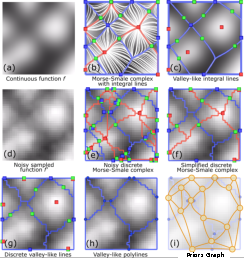
\includegraphics[width=0.6\textwidth]{./figures/mscbackground.pdf}
%  %}
%      \caption{ Morse-Smale complexes are defined for functions with continuous gradients {\bf(a-c)}. A smooth function {\bf(a)} can be partitioned based on the behavior of integral lines {\bf(b)}, with selected integral lines shown in white. This partition forms a cell complex, where integral lines within each cell share a common origin and destination. The 0-dimensional cells are  maxima (red), saddles (green), and minima (dark blue)), the 1-dimensional cells are formed by ascending (orange) and descending lines (light blue) from saddles (green), and 2-dimensional cells are bounded by 0- and 1-cells {\bf(b)}. Elements of this complex often form semantic features of interest in a scientific domain, such as valley-like lines {\bf(c)}. Real-world functions often come from noisy sources, and are available as samples on a grid {\bf(d)}. Discrete Morse-theory-based methods allow practical computation of Morse-Smale complexes {\bf(e)}, which encode both noise and discretization artifacts that may be simplified to recover the coarse-scale behavior of the function {\bf(f)}. The valley-like structures may be extracted from this complex {\bf(g)}, and converted to a set of priors between non-degree-2 vertices denoted the valley graph {\bf(h)}. The priors graph (yellow), {\bf(i)}, represents each prior as a vertex with edges between incident priors. }
%      \label{mscbackground}
%  \end{figure}
\fi
 





\end{document}
